%!TEX root = main-ugly.tex
Let $\tf A \in \LTV^{n,n}$ and $\tf B \in \LTV^{n,p}$, and consider the dynamical system mapping $\ell^n_{\infty,e} \times \ell^p_{\infty,e} \to \ell^n_{\infty,e}$ defined by
\begin{equation}
\tf x = \Sp\tf A\tf x + \Sp \tf B \tf u + \Sp \tf w, \ x_0 = 0.
\label{eq:dynamics}
\end{equation}
As $\Sp\tf A$ is strictly causal, the feedback interconnection defined by the dynamics \eqref{eq:dynamics} is well posed in the sense that $(I-\Sp\tf A)^{-1}$ exists as an operator from $\ell^n_{\infty,e} \times \ell^p_{\infty,e} \to \ell^n_{\infty,e}$ \cite{dahleh1994control}.  We emphasize that although we impose that $\A$ be $\ell_\infty$-stable, this does not imply that the dynamics \eqref{eq:dynamics} are themselves open-loop stable.  Rather, open-loop stability of the system is determined by the $\ell_\infty$ stability of the operator $(I-\Sp\tf A)^{-1}$.

Note that if $\tf A$ and $\tf B$ are memoryless and time invariant, i.e., if their matrix representations are block-diagonal $\tf A = \mathrm{blkdiag}(A,A,\dots)$, $\tf B = \mathrm{blkdiag}(B,B,\dots)$, then the system \eqref{eq:dynamics} reduce to the familiar finite-dimensional LTI system
\begin{equation}
x_{t+1} = A x_t + Bu_t + w_t, \, x_0 = 0,
\label{eq:lti-dynamics}
\end{equation}
where once again stability of the open-loop system is determined by the stability of the operator $(zI-A)^{-1}$ as opposed to the boundedness of the matrix $A$.

For LTI systems \eqref{eq:lti-dynamics}, the System Level Synthesis (SLS) framework \cite{wang2019system,anderson2019system} provides an appealing parameterization of all closed loop responses from $\tf w \to (\tf x, \tf u)$ achievable by a causal state-feedback $\ell_\infty$-stabilizing (equivalently internally stabilizing) LTI control law $\tf K$ such that $\tf u = \tf K \tf x$, as summarized in the following theorem.  We remind the reader that a controller $\tf K$ is $\ell_\infty$-stabilizing (equivalently internally stabilizing) if its interconnection with the system dynamics, as illustrated in Fig. \ref{fig:lti-interconnect}, defines an $\ell_\infty$-stable map from $(\tf w, \tf \delta_y, \tf \delta_u) \to (\tf x, \tf u, \what)$ (see III.A of \cite{wang2019system}).

\begin{figure}
\centering
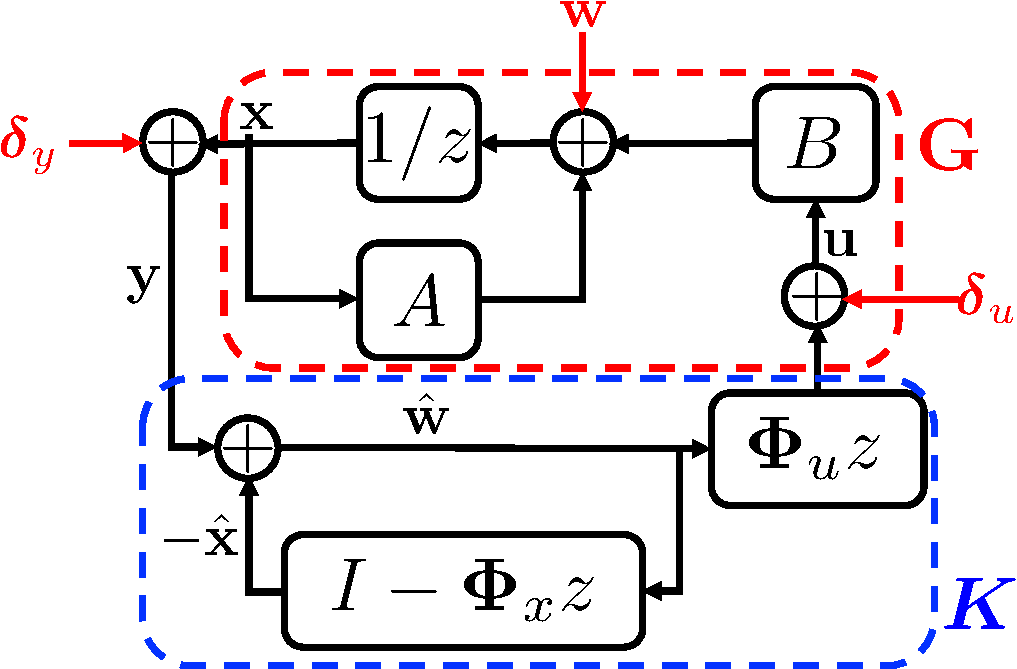
\includegraphics[width=.35\textwidth]{lti-interconnect}
\caption{The proposed $\ell_\infty$-stabilizing (equivalently internally stabilizing) state-feedback controller structure defined by equations \eqref{eq:lti-realization}.}
\label{fig:lti-interconnect}
\end{figure}

\begin{theorem}[Theorem 1, \cite{wang2019system}]\label{thm:lti-sls}
For the LTI system \eqref{eq:lti-dynamics} with causal state-feedback LTI control law $\tf u = \tf K \tf x$, the follwing are true:
\begin{enumerate}
\item The affine subspace defined by 
\begin{equation}
\begin{bmatrix} zI - A & - B \end{bmatrix} \begin{bmatrix} \Phix \\ \Phiu \end{bmatrix} = I, \, \ \Phix, \Phiu \in \frac{1}{z}\RHinf
\label{eq:lti-achievable}
\end{equation}
parameterizes all system responses
\begin{equation}
\begin{bmatrix} \tf x \\ \tf u \end{bmatrix} = \begin{bmatrix} \Phix \\ \Phiu \end{bmatrix} \tf w
\label{eq:lti-response}
\end{equation}
achievable by an internally stabilizing state-feedback controller $\tf K$.
\item For any transfer matrices $\left\{\Phix, \Phiu\right\}$ satisfying the constraints \eqref{eq:lti-achievable}, the control signal computed via\footnote{We note that due to the affine constraints \eqref{eq:lti-achievable}, $z\Phix-I$ is strictly causal, and thus feedback loop between $\tf{\hat x}$ and $\tf{\hat w}$ is well posed.}
\begin{equation}
\begin{array}{rcl}
\tf u &=& z\Phiu \tf{\hat w} \\
\tf{\hat w} &=& \tf x - \tf{\hat x}, \, \hat{w}_0 = 0, \\ 
\tf{\hat x} &=& (z\Phix - I)\tf{\hat w}
\end{array}
\label{eq:lti-realization}
\end{equation}
defines the control law $\uu = \Phiu\Phix^{-1}\x$, is internally stabilizing, and achieves the desired response \eqref{eq:lti-response}.
\end{enumerate}
\end{theorem}

Thus, in the case of LTI systems \eqref{eq:lti-dynamics}, the search for an optimal controller $\tf K$ can be converted to a search over system responses $\left\{\Phix,\Phiu\right\}$ constrained to lie in the affine space defined by equation \eqref{eq:lti-achievable}.  This fact, combined with the transparent mapping between the system responses and the corresponding controller implementation \eqref{eq:lti-realization}, has been successfully exploited for the synthesis of distributed optimal controllers for large-scale systems by imposing additional convex structural constraints, such as delay, sparsity, and locality subspace constriants, on the system responses and corresponding controller implementation \eqref{eq:lti-realization} -- we refer the reader to \cite{wang2014localized,wang2016localized,wang2018separable} for more details.

Another favorable feature of the parameterization defined in Theorem \ref{thm:lti-sls} is that it is provably stable under perturbations from the subspace \eqref{eq:lti-achievable}, as summarized in the following theorem from \cite{matni2017scalable}.

\begin{theorem}[Theorem 2, \cite{matni2017scalable}]\label{thm:lti-robust}
Let $(\Phixh,\Phiuh,\D)$ be a solution to
\begin{equation}
\begin{bmatrix} zI - A & - B \end{bmatrix} \begin{bmatrix} \Phixh \\ \Phiuh \end{bmatrix} = I - \D, \, \ \Phixh, \Phiuh \in \frac{1}{z}\RHinf.
\label{eq:lti-robust}
\end{equation}
If $(I-\D)^{-1}$ exists as an operator from $\ell^n_{\infty,e} \to \ell^n_{\infty,e}$, then the controller implementation \eqref{eq:lti-realization} defined in terms of the transfer matrices $\left\{\Phixh,\Phiuh\right\}$ achieves the closed loop responses
\begin{equation}
\begin{bmatrix}\tf x \\ \tf u \end{bmatrix} = \begin{bmatrix} \Phixh \\ \Phiuh \end{bmatrix}(I-\D)^{-1}\tf w,
\end{equation}
on the LTI system \eqref{eq:lti-dynamics}, and is internally stabilizing if and only if $(I-\D)^{-1} \in \RHinf$.
\end{theorem}
This parameterization has proved crucial in providing tractable approximations to non-convex distributed control problems \cite{matni2017scalable}, and in providing sub-optimality bounds for robust controllers as applied to learned systems \cite{dean2017sample}.  However, in these past works, very crude approximations based solely on small gain bounds and triangle inequalities were used to control the effects of the uncertain map $(I-\D)^{-1}$ on system stability and performance.  In this work we show that Theorems \ref{thm:lti-sls} and \ref{thm:lti-robust} can be extended to a more general setting that allows connections to well developed tools from the robust control literature \cite{khammash1990stability,dahleh1994control}.  Although we focus on $\mathcal{L}_1$ optimal control in this paper due to its favorable separability structure (see \S \ref{sec:extensions}), we expect these results to carry over naturally to the $\mathcal{H}_\infty$ setting.

\subsection{Necessary Conditions}
Here we characterize a set of affine constraints that the closed loop system responses of system \eqref{eq:dynamics} must satisfy if they are induced by a linear, causal, and $\ell_\infty$-stabilizing controller $\tf K : \ell^n_{\infty,e} \to \ell^p_{\infty,e}$ via the control law $\tf u = \tf K \tf x$.  In particular, a controller $\tf K$ is $\ell_\infty$-stabilizing if the interconnection illustrated in Fig. \ref{fig:simple-interconnect} is $\ell_\infty$-stable as a map from $(\tf w, \tf \delta_y, \tf \delta_u)\to (\x,\uu,\tf \beta)$, where $\tf \beta$ is any signal internal to the controller $\tf K$.

\begin{figure}
\centering
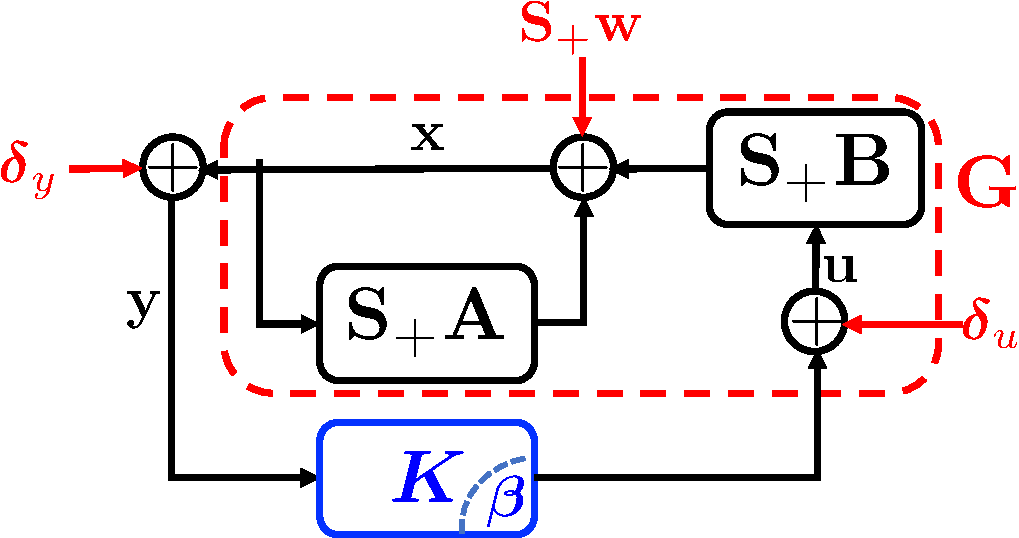
\includegraphics[width=.35\textwidth]{simple-interconnect}
\caption{A controller $\tf K$ is said to be $\ell_\infty$-stabilizing with respect to dynamics \eqref{eq:dynamics} if the illustrated interconnection is $\ell_\infty$-stable as a map from $(\tf w, \tf \delta_y, \tf \delta_u)\to (\x,\uu,\tf \beta)$, where $\tf \beta$ is any signal internal to the controller $\tf K$.}
\label{fig:simple-interconnect}
\end{figure}

\begin{proposition}\label{prop:necessity}
Let $\tf K: \ell^n_{\infty,e} \to \ell^p_{\infty,e}$ be a linear, causal, and $\ell_\infty$-stabilizing controller. 
%such that $(I-\Sp(\A+\B\K))^{-1}\Sp$ and $\K(I-\Sp(\A+\B\K))^{-1}\Sp$ are $\ell_\infty$-stable, i.e., let $\tf K$ be a linear causal controller such that closed loop maps from $\tf w \to (\tf x, \tf u)$ are $\ell_\infty$-stable.  
Then all maps taking $\tf w \to (\tf x, \tf u)$ achievable by such a $\tf K$ satisfy the constraints
\begin{equation}
\begin{aligned}
&\begin{bmatrix} I-\Sp\A & - \Sp\B\end{bmatrix}\begin{bmatrix} \Phix \\ \Phiu \end{bmatrix} = \Sp, \\ &\Phix, \Phiu \text{ strictly causal, linear, and $\ell_\infty$-stable.}
\end{aligned}
\label{eq:osls-achievable}
\end{equation}
\end{proposition}

\begin{proof}
Basic algebra shows that the map from $\tf w \to \x$ is given by $(I-\Sp(\A+\B\K))^{-1}\Sp$, and that the map from $\tf w \to \uu$ is given by $\K(I-\Sp(\A+\B\K))^{-1}\Sp$.  By assumption, both of these maps are $\ell_\infty$-stable,\footnote{That they are well posed is immediate as $\Sp(\A+\B\K)$ is strictly causal.} as $\tf K$ is an $\ell_\infty$-stabilizing controller.
%As $\Sp(\A+\B\K)$ is strictly causal, the feedback interconnection is well posed in the sense that $(I-\Sp(\A+\B\K))^{-1}$ exists as a map from $\ell^n_{\infty,e} \to \ell^n_{\infty,e}$.  
%By assumption, both $(I-\Sp(\A+\B\K))^{-1}$ and $\tf K(I-\Sp(\A+\B\K))^{-1}$ are $\ell_\infty$-stable. 
Defining
\[
\begin{bmatrix}
\Phix \\ \Phiu
\end{bmatrix} =
\begin{bmatrix} I \\ \K \end{bmatrix}(I-\Sp(\A+\B\K))^{-1}\Sp,
\]
it is easily verified that $\left\{\Phix,\Phiu\right\}$ satisfy constraint \eqref{eq:osls-achievable}.
\end{proof}
\begin{remark}
If $\A$ and $\B$ are LTI, and $\K$ is LTI, then so are $\{\Phix,\Phiu\}$, and all are uniquely characterized by their $z$-transforms.  Further the right shift operator $\Sp$, when restricted to $\LTI$, can be written as $\Sp=\frac{1}{z}I$.  In this case, constraint \eqref{eq:osls-achievable} simplifies to
\begin{equation}
\begin{bmatrix} I - \frac{1}{z}\A& -\frac{1}{z}\B \end{bmatrix} \begin{bmatrix} \Phix \\ \Phiu\end{bmatrix} = \frac{1}{z}I, \, \ \Phix, \Phiu \in \frac{1}{z}\RHinf,
\end{equation}
which can be viewed as a generalization of constraint \eqref{eq:lti-achievable} to LTI dynamics defined by dynamic operators $\A(z)$ and $\B(z)$.  Similarly, if $\A$ and $\B$ are memoryless and LTI, and $\K$ is LTI, then $\{\Phix,\Phiu\}$ are LTI, and constraint \eqref{eq:osls-achievable} simplifies to
\begin{equation}
\begin{bmatrix} I - \frac{1}{z}A & -\frac{1}{z}B \end{bmatrix} \begin{bmatrix} \Phix \\ \Phiu \end{bmatrix} = \frac{1}{z}I, \, \ \Phix, \Phiu \in \frac{1}{z}\RHinf,
\end{equation}
which is clearly equivalent to \eqref{eq:lti-achievable}.
\end{remark}

\subsection{Controller Implementation}
\begin{figure}
\centering
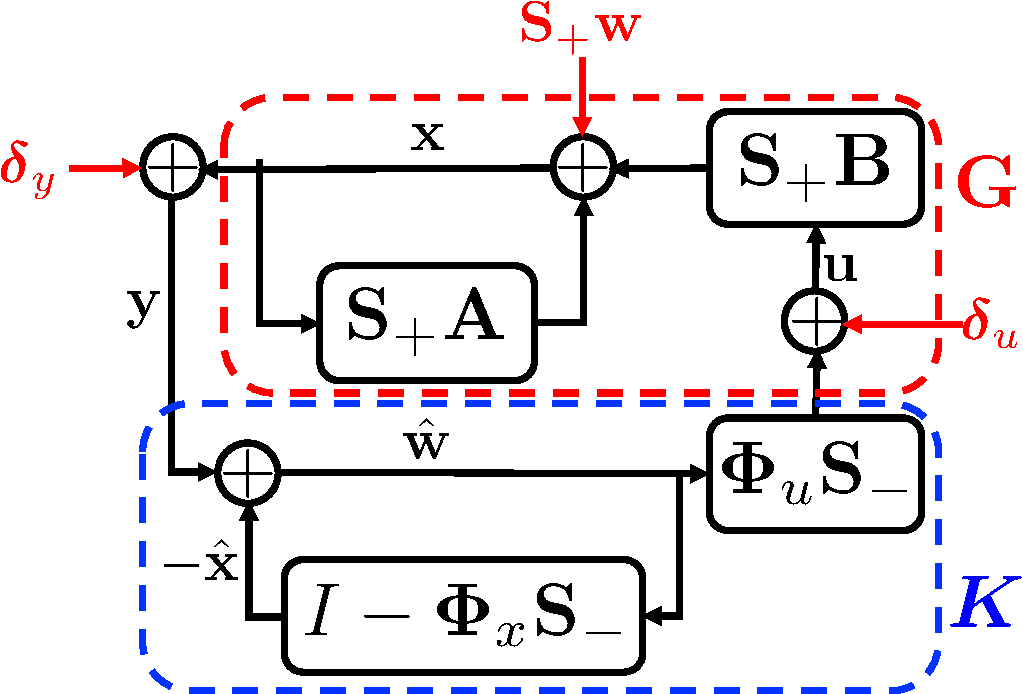
\includegraphics[width=.35\textwidth]{interconnect}
\caption{The proposed state-feedback controller structure defined by equations \eqref{eq:realization}.}
\label{fig:realization}
\end{figure}
We now show how to construct an internally stabilizing controller from any strictly causal, linear, and $\ell_\infty$-stable operators $\left \{\Phix,\Phiu\right\}$ satisfying constraint \eqref{eq:osls-achievable} that achieves the desired response from $\tf w \to (\tf x, \tf u)$.
\begin{proposition}\label{prop:sufficiency}
Let $\left\{\Phix,\Phiu\right\}$ satisfy constraint \eqref{eq:osls-achievable}.  Then the controller implementation shown in Fig. \ref{fig:realization}, described by the equations
\begin{equation}
\begin{array}{rcl}
\tf u &=& \Phiu \Sm \tf{\hat w}\\
\tf{\hat w} & = & \x - \tf{\hat x}, \, \hat{w}_0 = 0, \\
\tf{\hat x} &=& (\Phix\Sm-I)\tf{\hat w},
\end{array}
\label{eq:realization}
\end{equation}
is $\ell_\infty$-stabilizing.  In particular, the resulting map from $(\tf w, \tf \delta_y, \tf \delta_u) \to (\tf x, \tf u, \tf{\hat w})$ is $\ell_\infty$-stable, and achieves the desired closed loop response
\begin{equation}
\begin{bmatrix} \tf x \\ \tf u \end{bmatrix} = \begin{bmatrix} \Phix \\ \Phiu \end{bmatrix}\tf w.
\label{eq:response}
\end{equation}
\end{proposition}
\begin{proof}
From equations \eqref{eq:dynamics} and \eqref{eq:realization} (alternatively, from Fig. \ref{fig:realization}), we have that
\begin{equation}
\begin{array}{rcl}
\x &=& \Sp\A\x + \Sp\B\uu + \Sp \w, \ x_0 =0\\
\uu &=& \Phiu\Sm\what + \tf \delta_u\\
\what &=& \x + \tf \delta_y + (I-\Phix\Sm)\what, \ \hat{w}_0=0,
\end{array}
\label{eq:internal-stability}
\end{equation}
where we emphasize that $\hat{w}_0 = 0$ such that $\what$ is a strictly causal signal.  We first observe that the restriction of $(I-\Phix\Sm)$ to strictly causal signals is itself strictly causal, as the constraint \eqref{eq:osls-achievable} enforces that the block lower triangular matrix representation of $\Phix$ has identify matrices along its first block sub-diagonal, i.e., for $\Phix = (\Phi_x(i,j))_{i,j=0}^\infty$ the block lower triangular matrix representation of $\Phix$, we have that $\Phi_x(i,i-1)=I$ for all $i\geq 1$.  It therefore follows that the feedback loop between $\xhat$ and $\what$ is well posed.  By rote calculation, it follows from equation \eqref{eq:internal-stability} that the closed loop maps from $(\tf w, \tf \delta_y, \tf \delta_u) \to (\tf x, \tf u, \tf{\hat w})$ are given by
\begin{equation}
\begin{bmatrix}
\x \\ \uu \\ \what
\end{bmatrix} =
\begin{bmatrix} \Phix & \Phix(\Sm - \A) & \Phix\B \\
\Phiu & \Phiu(\Sm-\A) & I + \Phiu\B \\
\Sp & I - \Sp\A & \Sp \B
\end{bmatrix} \begin{bmatrix} \tf w \\ \tf \delta_y \\ \tf \delta_u \end{bmatrix}.
\end{equation}
By assumption, $\Phix$, $\Phiu$, $\A$, and $\B$ are all $\ell_\infty$-stable, and hence the interconnection illustrated in Fig. \ref{fig:realization}, and described by equations \eqref{eq:dynamics} and \eqref{eq:internal-stability} is $\ell_\infty$-stable.
\end{proof}

\begin{remark}
If $\A$ and $\B$ are memoryless and LTI, and $\K$ is LTI, then so are the system responses $\left\{\Phix,\Phiu\right\}$, and consequently the right and left shift operators $\Sp$ and $\Sm$ become $\frac{1}{z}I$ and $zI$, respectively, recovering the controller implementation \eqref{eq:lti-realization}.
\end{remark}

\subsection{Robust Operator System Level Synthesis}
Propositions \ref{prop:necessity} and \ref{prop:sufficiency} show that the parameterization of Theorem \ref{thm:lti-sls} can be extended to a class of dynamics described by bounded and causal linear operators in feedback with a causal linear controller.  We now show that this extension enjoys similar stability properties with respect to perturbations from the subspace \eqref{eq:osls-achievable}.

\begin{theorem}\label{thm:robust-sls}
Let $\A\in\LTV^{n,n}$ and $\B\in\LTV^{n,p}$, and suppose that $\left\{\Phixh,\Phiuh\right\}$ satisfy
\begin{equation}
\begin{aligned}
&\begin{bmatrix} I-\Sp\A & - \Sp\B\end{bmatrix}\begin{bmatrix} \Phixh \\ \Phiuh \end{bmatrix} = \Sp(I-\D), \\ 
& \Phix, \Phiu \text{ strictly causal, linear, and $\ell_\infty$-stable,}
\end{aligned}
\end{equation}
for $\D$ a strictly causal linear operator from $\ell^n_{\infty,e}\to \ell^n_{\infty,e}$.  Then the controller implementation \eqref{eq:realization} defined in terms of the operators $\left\{\Phixh,\Phiuh\right\}$ is well posed and achieves the following response
\begin{equation}
\begin{bmatrix} \x \\ \uu \end{bmatrix} = \begin{bmatrix}\Phixh\\ \Phiuh \end{bmatrix}(I-\D)^{-1}\w.
\label{eq:robust-response}
\end{equation}
Further, this interconnection is $\ell_\infty$-stable if and only if $(I-\D)^{-1}$ is $\ell_\infty$-stable.
\end{theorem}
\begin{proof}
As $\D$ is strictly causal by assumption, $I_\D:= (I-\D)^{-1}$ exists as a map from $\ell^n_{\infty,e} \to \ell^n_{\infty,e}$.  Going through a similar argument as that in the proof of Proposition \ref{prop:sufficiency}, we observe that
\begin{equation}
\scriptstyle
\begin{bmatrix}
\x \\ \uu \\ \what
\end{bmatrix} =
\begin{bmatrix} \Phix I_\D & \Phix I_\D(\Sm - \A) & \Phix I_\D \B \\
\Phiu I_\D& \Phiu I_\D(\Sm-\A) & I + \Phiu I_\D\B \\
\Sp I_\D & I_\D(I - \Sp\A) & I_\D\Sp \B
\end{bmatrix} \begin{bmatrix} \tf w \\ \tf \delta_y \\ \tf \delta_u \end{bmatrix}.
\end{equation}

Thus we see that the desired map \eqref{eq:robust-response} from $\w \to (\x,\uu)$ is achieved.  Further, as $\Phix$, $\Phiu$, $\A$, $\B$ are all $\ell_\infty$-stable by assumption, it follows that the $\ell_\infty$-stability of the map from $(\tf w, \tf \delta_y, \tf \delta_u) \to (\x, \uu, \what)$ is determined by the $\ell_\infty$-stability of $I_\D$, from which the result follows.
\end{proof}
